\usepackage{siunitx,booktabs,xcolor,xspace,multirow,graphicx,lipsum}
\usepackage[spanish,mexico,es-noindentfirst]{babel}
\usepackage[utf8]{inputenc}
\usepackage{tikz}
\usepackage{tikzsymbols}
\usepackage{subcaption}
\usepackage{charter}
\usetheme{Madrid}
\usepackage{tcolorbox}
\usepackage{hyperref}
\usepackage{animate}
\usepackage{transparent}

\usepackage[T1]{fontenc}
\usepackage[export]{adjustbox}
\usetikzlibrary{positioning}
\usefonttheme{serif}
\DeclareUnicodeCharacter{2212}{\textendash}

\setbeamertemplate{frametitle}{
	\begin{beamercolorbox}[wd=\paperwidth, ht=0.85cm, sep=0.25cm]{frametitle}
		\begin{tikzpicture}[remember picture,overlay]
			\node[anchor=north east] at (current page.north east) {
\includegraphics[height=0.65cm]{fig/aries.png}};
		\end{tikzpicture}
		\usebeamerfont{frametitle}\bfseries\insertframetitle
	\end{beamercolorbox}
}
\definecolor{lightshadygreen}{RGB}{204, 230, 255}
\setbeamercovered{transparent}
\setbeamertemplate{caption}[numbered]
\setbeamercolor{frametitle}{bg=lightshadygreen,fg=black}
\setbeamercolor{author in head/foot}{bg=lightshadygreen,fg=blue}
\setbeamercolor{title in head/foot}{bg=lightshadygreen,fg=blue}
\setbeamercolor{date in head/foot}{bg=lightshadygreen,fg=blue}
\setbeamercolor{titlelike}{parent=structure,bg=lightshadygreen,fg=black}
\setbeamertemplate{section in toc}[sections numbered]
\setbeamertemplate{subsection in toc}[subsections numbered]
\setbeamerfont{section in toc}{series=\bfseries}
\setbeamercolor{section in toc}{fg=black}
\setbeamercolor{caption name}{fg=black}
\setbeamerfont{caption name}{series=\bfseries}
\setbeamerfont{caption}{size=\small}
\setbeamercolor{bibliography entry author}{fg=black}
\setbeamercolor{bibliography entry title}{fg=black} 
\setbeamertemplate{section in toc}{\inserttocsectionnumber.~\inserttocsection\par}
\setbeamertemplate{subsection in toc}{\hspace{1.5em}\inserttocsectionnumber.\inserttocsubsectionnumber~\inserttocsubsection\par}

% Apply the custom color to the frametitle
\setbeamercolor{frametitle}{bg=lightshadygreen, fg=black}

\title[\textbf{Astro-AI Meeting}]{\textbf{Generative AI for Image Reconstruction in Intensity Interferometry: a First Attempt}}
\author[\textbf{Km Nitu Rai}]{\textbf{\underline{Speaker:}} Km Nitu Rai \vspace{0.01cm} \\ 
	{\scriptsize \underline{\textcolor{blue}{niturai201296@gmail.com}}} \\
	{\scriptsize {\textbf{\underline{Contributers:}} Km Nitu Rai, Yuri van der Burg, Soumen Basak, Prasenjit Saha, and Subrata Sarangi}} \\
	{\scriptsize \underline{\textbf{\tiny Presenting at}}} \\	
	{\scriptsize \underline{\textcolor{blue}{Astro-AI Meeting at IUCAA Pune}}}}

\date{\vspace{-1cm}\textbf{24th April, 2024}}

\renewcommand{\maketitle}{
	\begin{figure}[!htb]
		\centering
		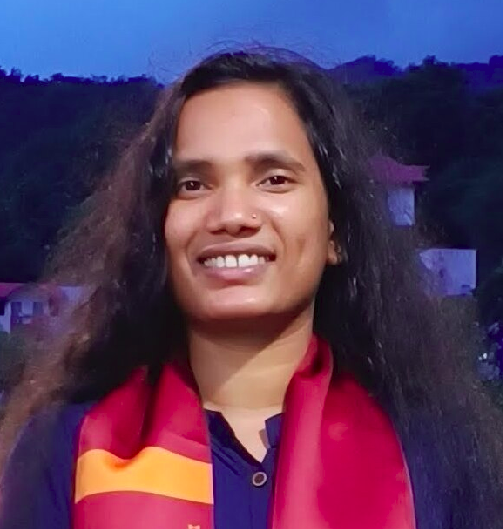
\includegraphics[height=2cm]{fig/team/Nitu.png}\hfill
		
\includegraphics[height=2cm]{fig/team/Yuri.png}\hfill
		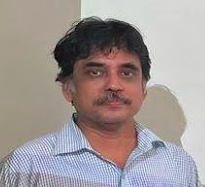
\includegraphics[height=2cm]{fig/team/Soumen.png}\hfill
		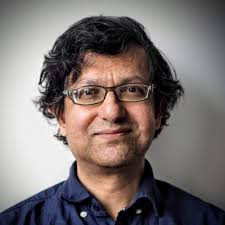
\includegraphics[height=2cm]{fig/team/Saha.jpeg}\hfill
		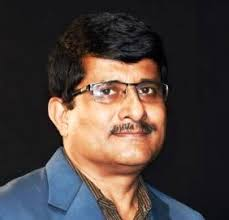
\includegraphics[height=2cm]{fig/team/Sarangi.jpeg}
	\end{figure}
	\vspace{-1cm}
	\titlepage
}

